eval(\chapter{Quick Start\label{sec:Quick-Start}}

The following sections give a short introduction in the main aspects
of using\noun{ EvA2}, explaining the possibilities accessible by the
GUI. Even if you want to use the API without the GUI, we recommend
to try some optimization runs through the GUI first, as it will help
to learn about the concepts used in the framework.


\section{Running \noun{EvA2}\label{sub:Quickly-Running-JavaEvA}}

To quickly test\noun{ EvA~2}, we recommend you download the jar-package
\emph{EvA2.jar} and start the GUI. The jar-file can be downloaded
from the \noun{EvA2} homepage%
\footnote{\url{http://www.ra.cs.uni-tuebingen.de/software/EvA2/}%
} \cite{EvA2HomePage}.

To start under GNU/Linux, you can just type:
\begin{quotation}
\texttt{\small \$ java -cp EvA2.jar eva2.gui.Main}{\small \par}
\end{quotation}
Note that ``\texttt{\$}'' stands for the command prompt, which needs
not to be typed. In the same or a similar way, you can start it on
all other platforms that support Java\noun{.} The Java option \emph{-jar}
is also possible with the base package of \noun{EvA2}, but does not allow adding
further jar-packages on the classpath. Therefore, we encourage using
the method given above.

If you want to work on the source code directly, note that it is also
vital to copy the resource folder to the directory where the compiled
class files are located. You can then again start the GUI or optimize
through the API (Sec.~\ref{sec:Using-the-API}). However we advise
you to learn to know the GUI a little before digging in the source
code.


\section{Some Words on the Words}

As \noun{EvA2} is mainly about Evolutionary and Heuristic Optimization,
some of the terms and notions are borrowed from the area and used
in this document. As they may not be familiar to all who want to use
the framework, we give a short summary here.

We aim at optimizing a target function without knowing much about
it, and find a certain position in the search space which minimizes
the function, called the \emph{solution}. During search, we use a
specific search strategy, the \emph{optimizer}, which usually looks
at several positions in parallel. Those are all \emph{potential solutions},
because we don't know the real one yet. For the potential solutions
we evaluate the target function. The value received is often called
\emph{fitness} in analogy to Darwin's Theory of Evolution, where ``the
fitter ones survive''. For the same reason, potential solutions are
sometimes called \emph{individuals}, and the set of potential solutions
stored by the optimizer at a time may be called \emph{the} \emph{population}.
Many of the implemented optimization strategies employ operators in
analogy to natural \emph{mutation}, \emph{crossover} and \emph{selection}. 

There is nothing mystical about that, and of course the analogy is
often exaggerated. Evolutionary Optimization is an algorithmic tool
that serves mostly technical purposes. That it works in a computer
is by no means a sign that we fully understand natural evolution or
can prove anything about it. This said, of course, we would never
doubt that natural evolution in fact works.

This document will not explain in detail how the implemented optimizers
work, as there is enough literature out there handling these topics.
We refer to Sec.~\ref{sec:Further-Reading} for suggestions on further
reading.




\section{Using the GUI\label{sub:Quickly-Using-GUI}}

From the GUI, also called the \noun{EvA} workbench, all important
components of an optimization run can be accessed and configured.
To change the optimization method, for example, click on the field
labeled with ``\emph{optimizer}'' and select the desired algorithm
from the drop-down menu. Basically, you thereby select a Java class
and create an instance, whose public properties are displayed in the
window immediately with their standard values. For your optimization
run, you may configure the parameter values directly through the input
fields. A short description will be displayed by tip-text above the
name of each parameter. If you just hit the ``\emph{Start}'' button,
an optimization will be started using the current settings. 

The \noun{EvA} GUI has two main tabs: the optimization parameter tab
and the statistics tab (Fig.~\ref{fig:Screenshots-workbench}), the
components of which will be summarized in the following.

\begin{figure}
\noindent \begin{centering}
\includegraphics[width=0.45\textwidth]{pics/screenshot-workb-2013}~~\includegraphics[width=0.45\textwidth]{pics/screenshot-stat-2013}
\par\end{centering}

\caption{Screenshots of the workbench window, with optimization (left) and
statistics (right) parameters.\label{fig:Screenshots-workbench}}
\end{figure}



\subsection{The Workbench Window\label{sub:The-Workbench-Window}}

The optimization parameters:
\begin{description}
\item [{\textit{Optimizer}}] Select the main optimization method. You can
choose between classical as well as evolutionary and swarm-based optimization
methods. For quick optimization, just use the standard values of the
parameters and try several different optimizers.
\item [{\textit{Post-processing~parameters}}] In some cases, post processing
of the results is desirable, e.g. if you want to improve the single
found solution by small hill climbing steps, or if you want to retrieve
more than one solution from a clustering optimization approach.
\item [{\textit{Problem}}] The instance of the target function to be optimized
is specified here. You can select from the benchmark problems delivered
with the package or inherit from the problem class yourself (Sec.~\ref{sec:Using-the-API}).
\item [{\textit{Random~Seed}}] As most algorithms in \noun{EvA2} incorporate
stochastic components, the random seed is critical for the specific
outcome of a run. For replicable results, set a seed value > 0. To
receive statistically relevant results, test several times with a
seed of 0, which means that the system time is used as seed for each
new run, or use the multi-run option.
\item [{\textit{Termination~Criterion}}] Set the criterion by which to
stop an optimization run, e.g. stop after \emph{n} fitness evaluations.
\end{description}
The Statistics parameters:
\begin{description}
\item [{\textit{Convergence~Rate~Threshold}}] Provided the target value
is zero, convergence is assumed if a value smaller than this threshold
is reached. For multi-run experiments, the number of hits is counted
using this criterion.
\item [{\textit{Field~Selection}}] The data fields to be displayed can
be selected. Typically, the current and best fitness are of most important,
but other fields such as average distance of candidate solutions may
be of interest. Since some data fields are complex types, such as
arrays, they are not plotted in the graph window but dumped to the
text window if marked. Depending on the problem and optimizer in use,
different data fields may be available. Specific information on the
data fields is given by tool tips in the application.
\item [{\textit{Number~of~Multi-runs}}] To achieve statistically meaningful
results on how well a certain optimizer works on a given problem,
set this number to do several runs in a row. The plot will be averaged,
while all intermediate data can be collected in an output file or
text window.
\item [{\textit{Output~All~Fields~As~Text}}] In some cases it is helpful
to show only selected data fields graphically but dump all data fields
to the text listeners, e.g., for external analysis.
\item [{\textit{Output~To}}] Textual information can be shown in a text
box, or redirected to a file, or both. The output file will be stored
to the current directory with a descriptive name containing the timestamp
of the start of the run.
\item [{\textit{Output~Verbosity}}] Select the verbosity of the textual
output, possible settings are ``no output'', ``final results'',
``k-th iterations'' and ``all iterations''. An iteration is usually
a generational cycle, meaning that for ``all iterations'', intermediate
data is printed after each generation.
\item [{\textit{Verbosity~Parameter~k}}] Define the interval parameter
for the ``k-th iterations'' setting of the output verbosity, by
which intermediate data is printed.
\end{description}
Finally, there are three buttons on top. \emph{``Description}''
shows some very general information on the main \noun{EvA} module.
The ``\emph{Start}'' button, as expected, starts an optimization
run using the parameters set, or multiple runs sequentially if \emph{multiRuns}
is set higher than one. During optimization, the ``\emph{Stop}''
button can abort the (multi-)run.


\subsection{The Plot Window}

\begin{figure}
\noindent \begin{centering}
\includegraphics[width=0.52\textwidth]{pics/screenshot-plot-window}
\par\end{centering}

\caption{Plot window comparing a simple (5,20)-ES and PSO on Rastrigin's after
10 runs each.\label{fig:The-plot-window}}
\end{figure}


During the optimization run, the progress of the solution is plottet
to a graph in a separate window (Fig.~\ref{fig:The-plot-window}).
Usually, the fitness of the best individual of every generation is
drawn in Y-direction along the number of function calls in X-direction.
Be aware that for multi-objective problems, only the first fitness
dimension is shown. The 2-dimensional multi-objective problem classes
have, however, a pareto-front viewer which displays the population
in the two fitness dimensions sequentially. For higher fitness dimensions
it is more practical to use external tools for visualization. Figure~\ref{fig:The-plot-window},
by the way, shows the fitness progress averaged over 10 runs of a
(5,20)-ES and a PSO strategy on Rastrigin's Problem: PSO converges
slower, but finds better results on the long run, while ES settles
earlier on higher plateaus. 

The visible buttons have the following functions:
\begin{description}
\item [{\emph{Clear}}] Remove all graphs from the plot window.
\item [{\textit{Log/Lin}}] Switch between linear and log-scaled view. Most
benchmark problems in \noun{EvA} are implemented with the minimum
fitness at zero, so that the log-scale view allows to compare and
analyze convergence behaviour in detail. Of course, if the target
fitness may become zero or negative, log-scale view is impossible.
\item [{\textit{Dump}}] Export the contained data to standard output. For
each graph, a column is created in the same order they were generated.
\item [{\textit{Export}}] Create the same output as \textit{Dump} and save
it to a file.
\item [{\textit{Save}\noun{~}\textit{as}\noun{~}\textit{PNG}}] Create
a PNG image of the plot window and save it to a file.
\end{description}

\subsection{Basic Optimization using \noun{EvA2}\label{sub:Basic-Optimization-GUI}}

To get a grip on \noun{EvA2} and what optimization means, it is best
to run some experiments on the implemented standard benchmarks. To
do that, start the GUI and select a benchmark problem, e.g. the F1-Problem
consisting in a simple hyper-parabola. Leave the post-processing deactivated.
Then choose an optimizer, such as Evolution Strategies with standard
parameters, set the termination criterion to EvaluationTerminator
with 10,000 fitness calls and push the ``Start Optimization'' button
at the top of the window. Two additional windows will now open up:
the plot window with a fitness graph, and a text box displaying the
optimization progess in textual form. The final result will be printed
into the text box at the end of the run, as well.

If you play around with some optimizer settings, e.g. you try different
values for $\mu$ and $\lambda$ or activate the plusStrategy checkbox,
you will notice changing performance of the ES. On problems within
discrete space, such as the B1-benchmark problem, for example, a Genetic
Algorithm is often superior to an Evolution Strategy. You can try
this if you clear the plot window, select the B1-problem and run the
ES a few times. Now, switch to the Genetic Algorithm and run the optimization
a few more times.

Notice, however, that by changing from the F1-problem to the B1-problem,
the internal representation of individuals may change. As B1 is a
typical binary problem, it uses GAIndividuals by default, which are
based on binary vectors, while F1 uses double vectors. Be aware, that
not all optimizers in \noun{EvA2} are built to work on all types of
indviduals.


\subsection{Post-Processing\label{sub:Post-Processing}}

To see how post processing works, you can select the \emph{FM0Problem}
from the problem list, which is a simple target function with a global
and a local optimum. Select the \emph{ClusterBasedNiching} algorithm
as the optimizer. Now click on the \emph{postProcessingParams} and
activate them. For a clustering distance of $\sigma=0.1$ and $\approx5,000$
hill climbing steps, the optimizer should print out just a few solutions
in the text box, the first of which hopefully are the optima near
(1.7/0) and (-1.44/0).

Post-processing serves mainly two purposes: filter redundant solutions
and refine the search results. Redundant solutions occur naturally
in population-based heuristics. The optimizer handles several potential
solutions in parallel, and it is hoped that they all converge on the
global optimum during the run. Or for multi-modal problems which have
several local optima, it can be desirable to have parts of the population
converge in different areas of the solution space. In any case, one
usually wants to retrieve \emph{the} solution set or a refined global
optimum. For this purpose, we employ a clustering approach which takes
the whole solution set and merges similar solutions to an associated
subset. For each of these bulks, only the best individual is returned
in the filtered solution set. 

\begin{figure}
\noindent \begin{centering}
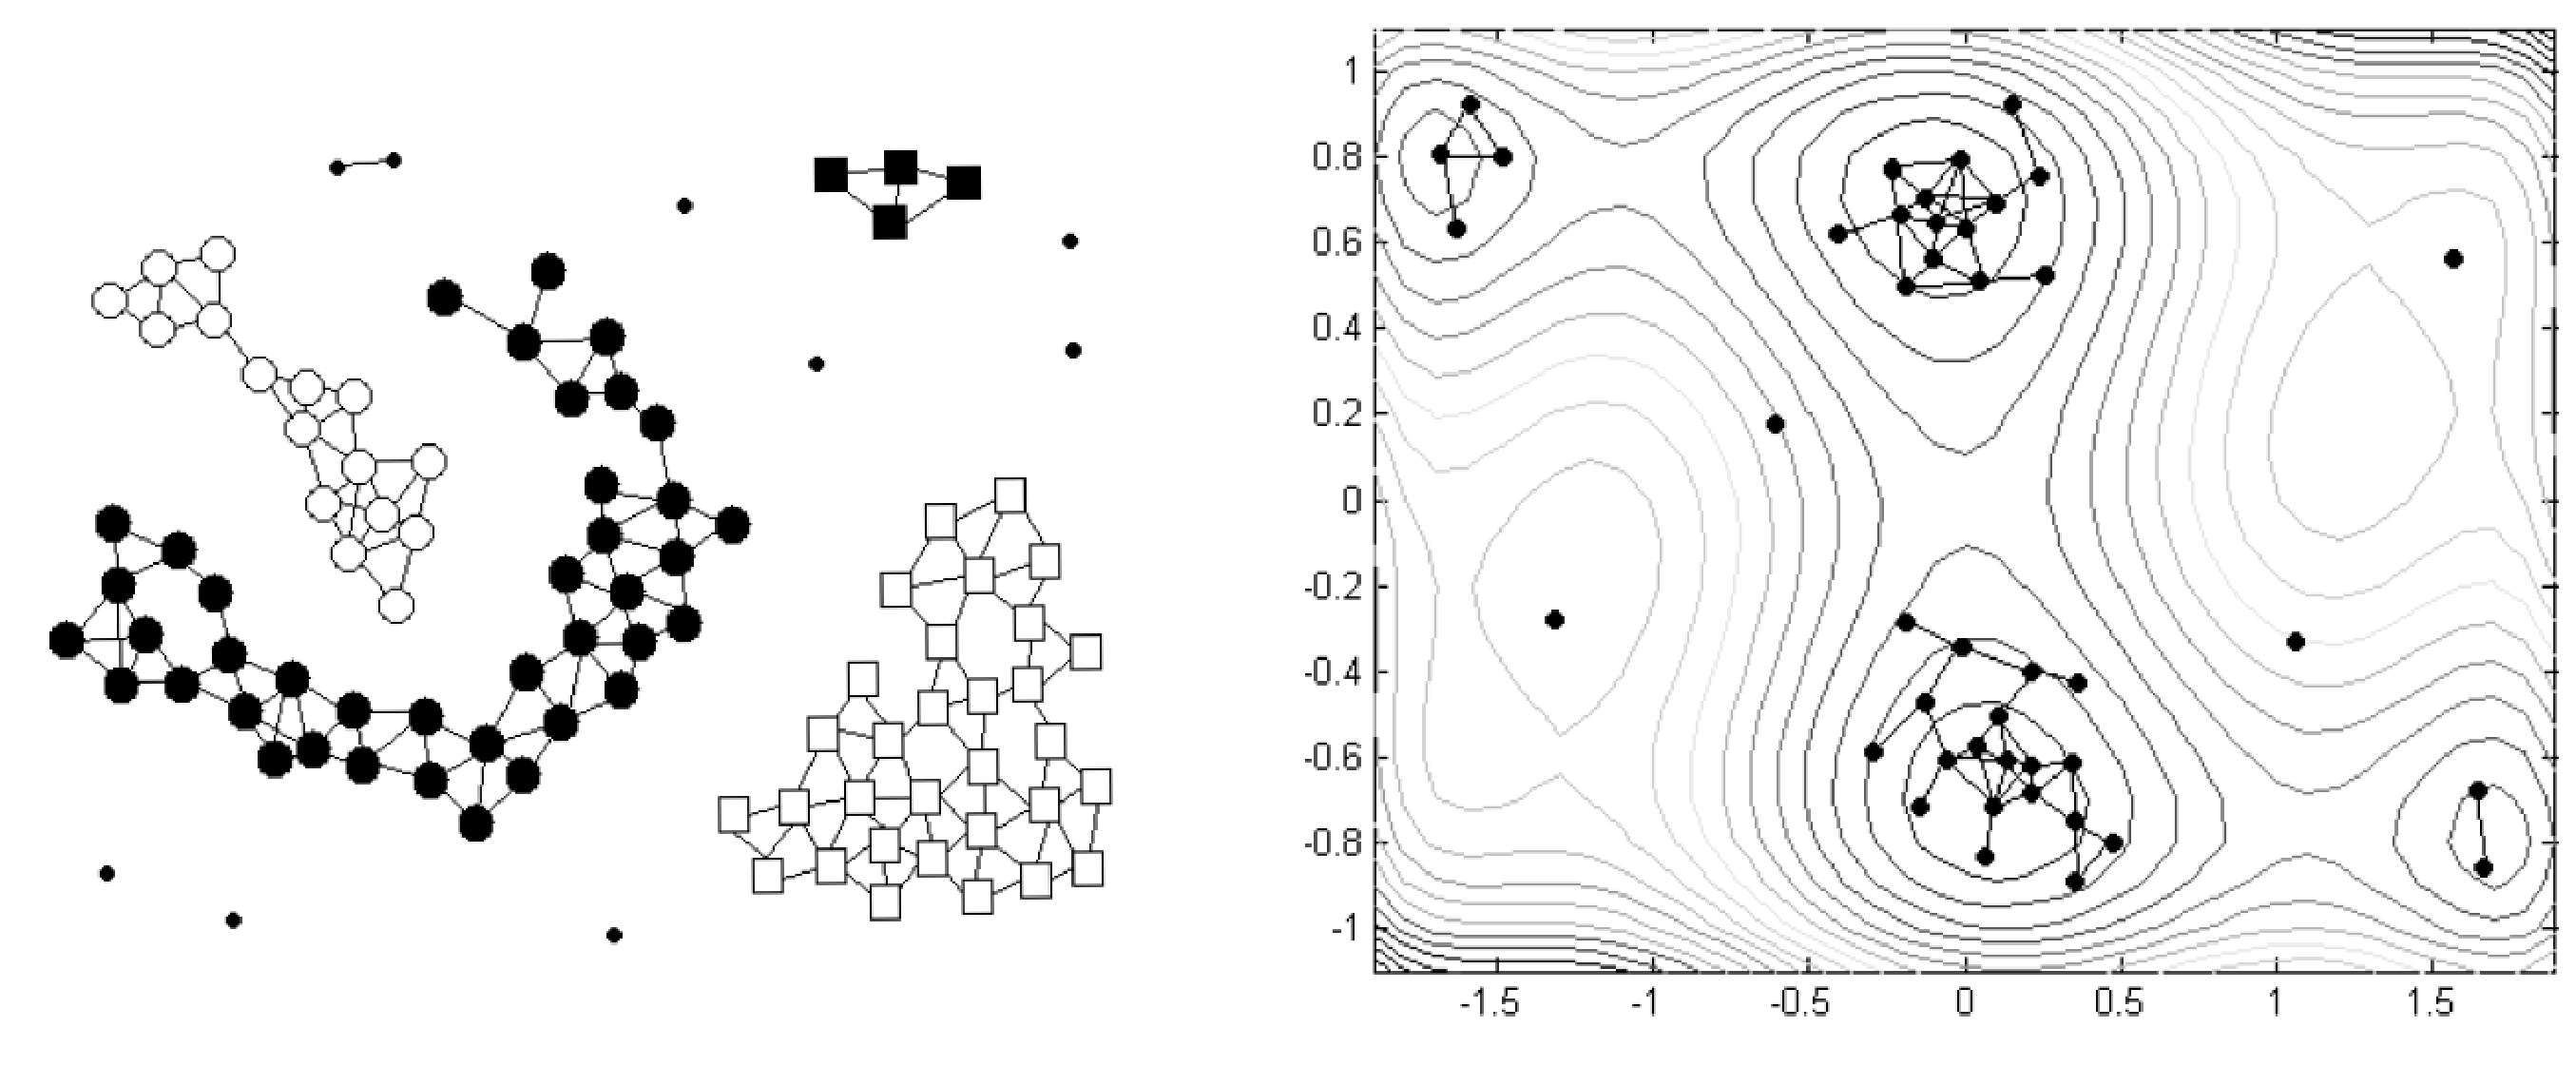
\includegraphics[width=0.8\columnwidth]{pics/cluster-graph}
\par\end{centering}

\caption{Examples for density based clustering (Streichert et al. \cite{streichertClustering03}).\label{fig:Density-based-clustering.}}
\end{figure}


Of course the size of this filtered set depends on the degree of convergence
in the original set and on the clustering criterion. We employ density
based clustering \cite{ester96density}, which associates any two
individuals which have a distance of less than the clustering parameter
$\sigma$ (Fig.~\ref{fig:Density-based-clustering.}). This is an
intuitive approach that does not require a predefined number of clusters,
in contrast to k-means, for example. By defining $\sigma$, you thus
define the resolution you grant your solution set.

As the solution set always contains the last state of the heuristic
optimization, one may hope that it is converged. But of course often
it is not fully converged, or maybe the strategy even rediversifies
the population from time to time, meaning that some part of the set
it is converged while other individuals are freshly initialized and
thus by no means optimal. So after filtering out redundancy, you might
also want to refine the returned set a little. This can be done directly
by Hill Climbing (HC) in the post-processing step by setting \emph{postProcessSteps}
to the number of evaluation calls you want to invest in the refinement.%
\begin{comment}
Question here: what is a hill climber?
\end{comment}


If you set $\sigma$ for clustering and performed hill climbing, then
there will be another clustering step right after the HC process,
to remove redundancy that emerged by the additional HC optimization.


\section{Additional Packages}

To add additional packages to use them with the \noun{EvA2} base package,
you can just add them to the class path. For instance, to use the
additional ``Probs'' package containing a larger set of benchmark
problems, place them both in your working directory and type (GNU/Linux):
\begin{quotation}
\texttt{\small \$ java -cp EvA2.jar:EvA2Probs.jar eva2.gui.Main}{\small \par}
\end{quotation}
You should now be able to select from a larger set of optimization
problems in the GUI. Note that different platforms use different characters
as path separators (':' in GNU/Linux). To add your own classes to
the \noun{EvA2} framework (see Sec.~\ref{sec:Quickly-Adding-Your-Problem}),
you need to add your local development path to the classpath, for
example:
\begin{quotation}
\texttt{\small \$ java -cp EvA2.jar:EvA2Probs.jar:/home/username/OwnClassDir
\textbackslash{}}{\small \par}

\texttt{\small eva2.gui.Main}{\small \par}
\end{quotation}
Note that \noun{EvA2} will search all classpath entries for compatible
classes, so you should only add those packages which are really required.
For your own additional packages, this also means that, if you want
your extensions (e.g. own problem implementations or operators) to
be displayed in the \noun{EvA~2} GUI, they have to be assigned the
same package tree as the associated \noun{EvA2} operators. Check Sec.~\ref{sec:Using-the-API}
on more details.
